\documentclass[10pt,twocolumn,letterpaper]{article}

\usepackage{cvpr}
\usepackage{times}
\usepackage{epsfig}
\usepackage{graphicx}
\usepackage{amsmath}
\usepackage{amssymb}

% Include other packages here, before hyperref.
\usepackage{booktabs}

% If you comment hyperref and then uncomment it, you should delete
% egpaper.aux before re-running latex.  (Or just hit 'q' on the first latex
% run, let it finish, and you should be clear).
\usepackage[breaklinks=true,bookmarks=false]{hyperref}

\cvprfinalcopy % *** Uncomment this line for the final submission

\def\cvprPaperID{****} % *** Enter the CVPR Paper ID here
\def\httilde{\mbox{\tt\raisebox{-.5ex}{\symbol{126}}}}

%\ifcvprfinal\pagestyle{empty}\fi
\setcounter{page}{1}
\begin{document}

%%%%%%%%% TITLE
\title{Domain-Adapted GPS Prediction for Italian Landscapes\\
via Parameter-Efficient Fine-Tuning of GeoCLIP}

\author{Amirhosein Arabhaji\\
{\tt\small amirhosein.arabhaji@studenti.unipd.it}
\and
Davide Sut\\
{\tt\small davide.sut@studenti.unipd.it}
}

\maketitle

%%%%%%%%% ABSTRACT
\begin{abstract}
We present a parameter-efficient approach to fine-tune
GeoCLIP, a CLIP-based geo-localization model,
for predicting GPS coordinates from photographs taken in Italy.
Starting from a pretrained 440M-parameter backbone, we inject Low-Rank
Adaptation (LoRA) adapters into all four attention projection
matrices of the Vision Transformer encoder, replace GeoCLIP's gallery-retrieval
head with a direct coordinate-regression head, and update only 1.4\% of the
weights.
We train on 111{,}787 images from the OpenStreetView-5M
(OSV5M) dataset filtered to Italy's borders via a polygon boundary
test, using a combined Haversine and L1 regression loss augmented with a land-aware penalty
that discourages predictions in the open sea.
Because fair and reproducible comparison is central to this work, we evaluate
every model, including both baselines and fine-tuned variants, through a single
inference-and-metrics pipeline on the fixed OSV5M test set of 1{,}397 images.
Our best model (V3.3 with test-time augmentation) achieves a median
error of 110.8~km and 73.6\% of predictions within 200~km, compared to
538.3~km / 24.6\% for the unmodified GeoCLIP baseline and 245.2~km / 42.8\% for
GeoCLIP restricted to an Italy-only retrieval gallery.
Against this stronger, Italy-constrained baseline our model still cuts median
error by 55\% (245.2$\to$110.8~km), showing the gain is not an artifact of
comparing against an unconstrained global gallery.
Macro-region classification accuracy improves from 63.5\% to 80.2\%.
An ablation traced through the same pipeline shows how dataset scale, LoRA
capacity, adapter scope, and test-time augmentation each contribute.
\end{abstract}

%%%%%%%%% BODY TEXT
\section{Introduction}

Visual geo-localization, the task of predicting the geographic location
depicted in a photograph, has applications in navigation, social-media
analysis, forensic verification, and cultural heritage documentation.
General-purpose models such as PlaNet~\cite{planet} and
GeoCLIP~\cite{geoclip} achieve impressive worldwide coverage, but their
performance in specific countries often lags behind what dedicated domain
adaptation can achieve.

Italy is a compelling target for regional geo-localization.
Its diverse landscape spans Alpine mountains, Mediterranean coastlines, historic
urban centers, and rural agricultural areas, all within a compact bounding box
($35.4$--$47.2^\circ$N, $6.6$--$18.8^\circ$E).
A practical geo-localization system for Italy could support tourism, cultural
heritage research, and automated geo-tagging of social-media photographs.

Our first attempts fine-tuned GeoCLIP by directly unfreezing the last Vision
Transformer (ViT) layers. Applying a standard learning rate ($10^{-4}$) to those
layers produced behavior consistent with catastrophic
forgetting~\cite{catastrophic_forgetting}, aggressively overwriting the
fine-grained feature detectors acquired during global pretraining.
This motivated a shift to parameter-efficient adaptation: we freeze the ViT
transformer blocks and inject LoRA adapters~\cite{lora} whose weight matrices
start at zero and grow only to capture Italy-specific signals, while additionally
training the visual projection and image-encoder MLP as lightweight
domain-adaptation components.

Beyond the model, this paper emphasizes \emph{evaluation consistency}.
Comparing a regression model with a retrieval model requires care because
GeoCLIP predicts the nearest entry in a fixed gallery of GPS candidates, most of
which lie outside Italy, whereas our regression head is structurally confined to
Italy. To ensure a fair comparison, we evaluate GeoCLIP both with its full global
gallery and with a gallery restricted to Italy, alongside the zero-shot
StreetCLIP~\cite{streetclip} retriever, and run all of them, plus every
fine-tuned checkpoint, through one shared inference-and-metrics pipeline on the
identical test set. All reported quantitative results and figures are produced
using this shared evaluation pipeline.

\noindent\textbf{Main contributions:}
\begin{itemize}
\itemsep0.2em
\item A parameter-efficient fine-tuning pipeline that converts GeoCLIP's
      retrieval design into direct GPS regression, updating only 1.4\% of a
      442M-parameter backbone.
\item A differentiable land-aware penalty loss designed to discourage
      off-coast predictions along Italy's extensive coastline.
\item A single unified evaluation harness that measures pretrained baselines
      (global gallery, Italy-only gallery, StreetCLIP) and every fine-tuned
      version identically, resolving the inconsistency of comparing a
      regressor to differently-configured retrievers.
\item A version-by-version ablation and region-level analysis on the fixed
      OSV5M Italy test set, showing an 87\% reduction in mean error and a
      macro-region classification accuracy of 80.2\%.
\end{itemize}

\section{Related Work}

\noindent\textbf{Image geo-localization.}
Hays and Efros~\cite{im2gps} showed that scene statistics carry a geographic
signal strong enough for continent-level retrieval.
PlaNet~\cite{planet} trained a CNN classifier over a discretized S2 cell grid,
achieving scalable worldwide localization.
Transformer-based approaches~\cite{translocator} leverage the global receptive
field of self-attention for scene-level cues.
Our work differs in that we target a single country through regression rather
than classification, preserving metric GPS coordinates.

\noindent\textbf{GeoCLIP.}
Vivanco Cepeda~\etal~\cite{geoclip} align CLIP image embeddings with location
encodings derived from random Fourier features of GPS coordinates via
contrastive pretraining on 100M image-GPS pairs.
At inference, images are ranked against a gallery of GPS candidates.
This gallery-based design is strong for worldwide localization but is not
optimized for dense intra-country coverage: only about 4{,}448 of its 100K
gallery cells fall inside Italy, motivating our regression approach.

\noindent\textbf{Parameter-efficient fine-tuning.}
LoRA~\cite{lora} adds low-rank adapter matrices $\mathbf{BA}$ (initialized
with $\mathbf{B}=\mathbf{0}$) in parallel with frozen weight matrices,
keeping the original embedding space intact.
Hu~\etal showed that rank-8 adapters match full fine-tuning on NLP benchmarks
while updating $<1\%$ of the parameters.
The PEFT library~\cite{peft} provides turnkey LoRA support for Hugging Face
transformers.

\noindent\textbf{StreetCLIP.}
Haas~\etal~\cite{streetclip} present StreetCLIP, a generalized zero-shot
learner for open-domain image geolocalization.
GPS candidates are encoded as text prompts and the nearest match to the image
embedding is returned.
On our Italy-constrained gallery (50K OSV5M train points encoded as text),
StreetCLIP reaches a median error of 438.8~km on OSV5M Italy, illustrating
that general zero-shot geolocalization does not substitute for domain-specific
adaptation.

\noindent\textbf{OSV5M.}
Astruc~\etal~\cite{osv5m} release five million geo-tagged street-view images
from OpenStreetMap contributors worldwide with a fixed train/test split.
Unlike landmark-centric GLDv2~\cite{gldv2}, OSV5M covers everyday roads,
intersections, and rural areas, making it substantially better suited for
regional geo-localization.

\section{Dataset}

\subsection{OpenStreetView-5M Italy Subset}
\label{sec:polygon}

We filter OSV5M~\cite{osv5m} to images inside Italy's borders using a
point-in-polygon test against a Natural Earth Italy boundary (via a prepared
\texttt{shapely} geometry, buffered 0.02$^\circ$ to keep coastal points), rather
than the coarser $35.4$--$47.2^\circ$N, $6.6$--$18.8^\circ$E bounding box, which
is used only as an outer pre-filter and as the regression target range in
\S\ref{sec:method}. This excludes points that fall inside the bounding box but
outside Italy (e.g., in neighboring countries or the sea), yielding 111{,}787
training images and 1{,}397 test images.
The test split is the fixed OSV5M partition; it is never used during training
or model selection, and it is the sole evaluation set for all quantitative
results in this paper.
For development, we split the training pool 85/15 (\texttt{random\_state=42}),
stratified by macro-region from V3.2 onward to prevent the Nord-heavy pool from
over-representing northern Italy in the validation set.

\noindent\textbf{Regional distribution.}
We use Italy's standard statistical macro-regions: Nord (North), Centro
(Center), and Sud/Isole (South and Islands).
The training pool skews north: Nord 57.6\%, Sud/Isole 23.1\%, Centro 19.3\%.
The test set presents the opposite skew: Sud/Isole 734 images (52.5\%), Nord 343
(24.6\%), Centro 320 (22.9\%).
This mismatch partially explains why Sud/Isole recall (74.7\%) trails Nord
(98.3\%) in the fine-tuned model (\S\ref{sec:region}).

\subsection{Legacy GLDv2 Experiments}

Two preliminary versions (V1, V2) used an Italy subset of GLDv2~\cite{gldv2}
(\raise.17ex\hbox{$\scriptstyle\sim$}34K landmark images after CLIP-fingerprint
deduplication). GLDv2's heavy bias toward famous monuments gave poor sub-city
precision, motivating the switch to OSV5M. We report GLDv2 numbers only briefly
for completeness (\S\ref{sec:gldv2}); they are on a different test set and are
not comparable to the OSV5M results that form the body of this paper.

\subsection{IM2GPS3k Italy Subset}
\label{sec:im2gps-dataset}

For a cross-dataset generalization check (\S\ref{sec:im2gps}), we additionally
use IM2GPS3k~\cite{im2gps}, the $\sim$3,000-image worldwide test benchmark of
Hays and Efros, filtered to Italy with the same polygon boundary test used for
OSV5M (\S\ref{sec:polygon}). This yields 110 images, predominantly landmark and
tourist-scene photographs, in contrast to OSV5M's everyday street-level
coverage. IM2GPS3k is never used for training or model selection; it serves
only as an out-of-distribution evaluation set.

\subsection{Preprocessing and Augmentation}

For validation and inference, images are resized to $224\times224$.
During training we apply random crop ($256\to224$), horizontal flip ($p=0.5$),
color jitter (brightness/contrast $\pm0.3$, saturation $\pm0.2$, hue $\pm0.05$),
random rotation ($\pm15^\circ$), and random grayscale ($p=0.05$).
All images are normalized with the OpenAI CLIP mean $[0.481, 0.458, 0.408]$ and
standard deviation $[0.269, 0.261, 0.276]$. Augmentations were fixed across all
versions to avoid confounding train/test distribution shifts.

\section{Method}
\label{sec:method}

\subsection{From Retrieval to Regression}

GeoCLIP~\cite{geoclip} consists of a CLIP ViT-Large/Patch14 image encoder
and a location encoder that maps GPS coordinates to 512-d vectors.
At inference time, it performs nearest-neighbor lookup over a gallery of GPS
candidates.
We discard the location encoder and the gallery entirely and attach a direct
regression head to the image features. Our fine-tuned model performs
\emph{no} gallery lookup at any stage; it emits a continuous $(\phi,\lambda)$
pair. In our experiments, the gallery is used only by the pretrained retrieval
baselines described in \S\ref{sec:baselines} and not by our regression model.

\subsection{Adaptation Strategy}

The ViT transformer blocks are frozen throughout training.
LoRA adapters are injected into the attention projection matrices of every
ViT encoder layer, allowing the attention mechanism to adapt without modifying
the frozen weights. The adapter update is
\begin{equation}
\Delta\mathbf{W} = \frac{\alpha}{r}\,\mathbf{B}\mathbf{A},\quad
\mathbf{A}\in\mathbb{R}^{r\times d},\;
\mathbf{B}\in\mathbb{R}^{d\times r},\;
\mathbf{B}=\mathbf{0}\text{ at init},
\label{eq:lora}
\end{equation}
where $r$ is the rank and $\alpha$ the scaling factor.
Additionally, the visual projection ($512\times768$) and image-encoder MLP are
trained as a lightweight domain-adaptation bottleneck between the frozen ViT
features and the regression head.
In V3.2/V3.3 the LoRA targets expand from $\{q,v\}$ to all four projections
$\{q,k,v,\mathrm{out}\}$ and the rank doubles from 8 to 16.
Table~\ref{tab:params} summarizes trainable parameter counts.

\begin{table}[t]
\centering\small
\begin{tabular}{@{}lcccc@{}}
\toprule
Ver. & LoRA targets & $r$ & Trainable & \% \\
\midrule
V1   & None (2 ViT layers) & --  & 28.1M & 6.4 \\
V2   & q, v          &  8  & $\approx$2M  & 0.5 \\
V3.1 & q, v          &  8  & $\approx$2M  & 0.5 \\
V3.2 & q, k, v, out  & 16  & 6.1M  & 1.4 \\
V3.3 & q, k, v, out  & 16  & 6.1M  & 1.4 \\
\bottomrule
\end{tabular}
\smallskip
\caption{Trainable parameter counts. V3.2/V3.3 breakdown: 3.15M LoRA adapters,
0.79M visual projection, 0.98M MLP, 1.19M regressor.}
\label{tab:params}
\end{table}

\subsection{Regression Head}

The 512-d CLIP pooled feature passes through
$512 \!\to\! 1024 \!\to\! 512 \!\to\! 256 \!\to\! 2$,
with BatchNorm + GELU + Dropout ($p{=}0.3,0.2,0.1$) between layers and a final
Sigmoid. The output $\hat{y}\in[0,1]^2$ maps to coordinates by
\begin{align}
\hat{\phi} &= \hat{y}_0\cdot(\phi_{\max}-\phi_{\min})+\phi_{\min}, \\
\hat{\lambda} &= \hat{y}_1\cdot(\lambda_{\max}-\lambda_{\min})+\lambda_{\min},
\end{align}
with $[\phi_{\min},\phi_{\max}]=[35.4^\circ,47.2^\circ]$ and
$[\lambda_{\min},\lambda_{\max}]=[6.6^\circ,18.8^\circ]$.
The Sigmoid confines every prediction to Italy's bounding box by construction.

\subsection{Loss Function}

\noindent\textbf{Base loss.} We combine an L1 term (normalized coordinates) with
a Haversine distance term (km, divided by 1000 for stability):
\begin{equation}
\mathcal{L}_{\text{base}}
  = 0.05\,\mathcal{L}_{L1}(\hat{y},y)
  + 0.95\,\mathcal{L}_{\text{Hav}}(\hat{p},p).
\end{equation}
The 95:5 weighting prioritizes the geographically meaningful metric while the L1
term provides a smooth gradient near the optimum.

\noindent\textbf{Land-aware penalty (V3.1--V3.3).}
Italy's long coastline makes many ambiguous scenes (harbors, beaches) prone to
offshore predictions. We add a differentiable penalty that is zero on land or
within $d_{\text{buf}}=25$~km of the coast and ramps linearly to 1.0 at
$d_{\text{scale}}=150$~km offshore:
\begin{equation}
\mathcal{L}_{\text{land}}(\hat{p})
  = \frac{1}{B}\sum_{i=1}^{B}
    \mathrm{clip}\!\left(\tfrac{d_i - d_{\text{buf}}}{d_{\text{scale}}},0,1\right),
\end{equation}
where $d_i$ is the distance from the $i$-th prediction to the nearest land pixel.
The grid is precomputed at $300\times300$ over Italy using
\texttt{global\_land\_mask} and \texttt{scipy}'s distance transform, and sampled
differentiably via \texttt{F.grid\_sample}. The combined loss is
$\mathcal{L} = \mathcal{L}_{\text{base}} + 0.20\,\mathcal{L}_{\text{land}}$.

\subsection{Test-Time Augmentation (V3.3)}

At inference we average GPS predictions over six deterministic views: standard
resize; horizontal flip; center-crop from 256~px; flipped center-crop; a fixed
brightness/contrast increase; and a fixed $+10^\circ$ rotation. Averaging
coordinates reduces variance with no retraining.

\begin{figure*}[t]
  \centering
  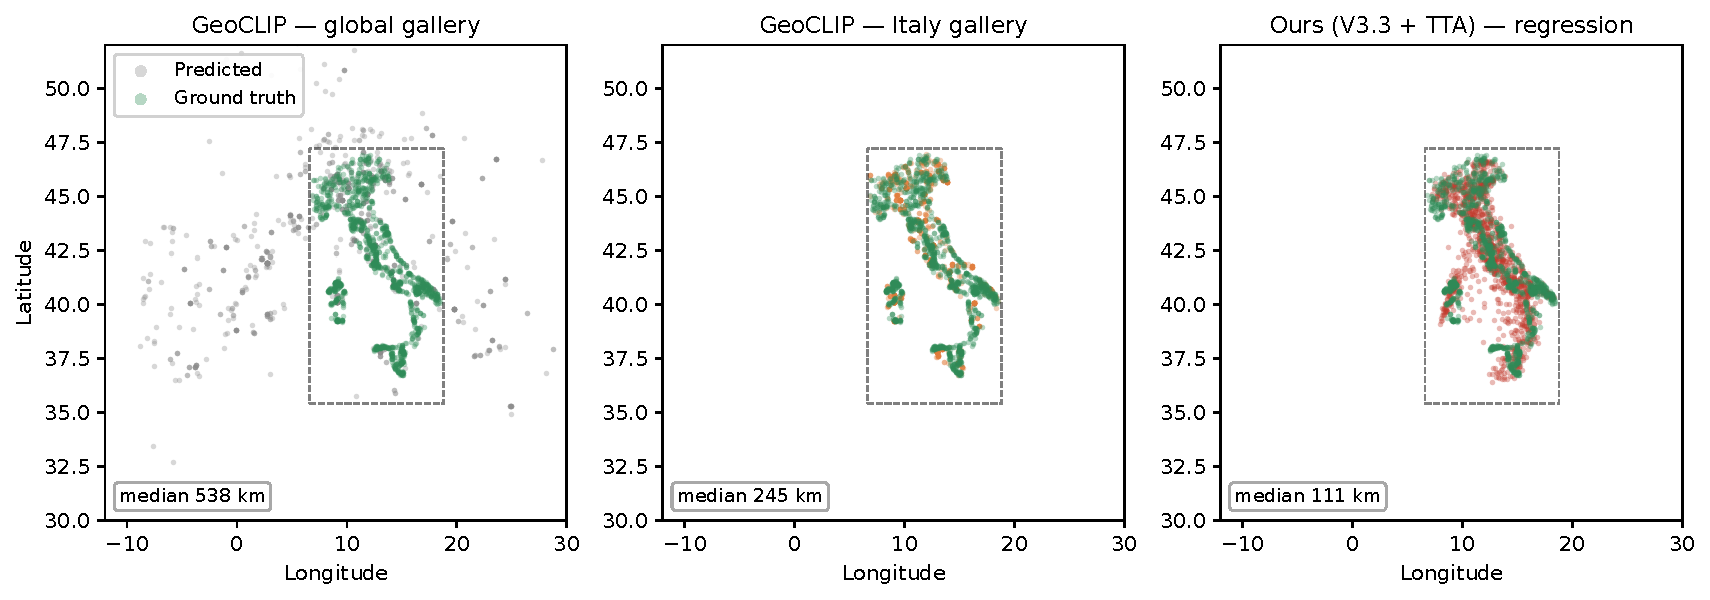
\includegraphics[width=0.99\linewidth]{./charts/scatter_3panel}
  \caption{Predicted (colored) vs.\ ground-truth (green) GPS coordinates on the
  OSV5M Italy test set (1{,}397 images); dashed box is Italy's bounding box.
  \textbf{Left:} pretrained GeoCLIP with its full global gallery scatters
  predictions across Europe and beyond. \textbf{Center:} restricting GeoCLIP's
  gallery to Italy forces in-country answers but remains coarse. \textbf{Right:}
  our regression model (no gallery) clusters tightly on the true locations.
  Median errors are annotated per panel.}
  \label{fig:scatter}
\end{figure*}

\section{Experiments}

\subsection{Unified Evaluation Protocol}
\label{sec:baselines}

All models are evaluated by one shared harness that loads the fixed OSV5M test
set, runs inference, and computes Haversine error and threshold accuracies
identically. We compare our fine-tuned checkpoints against four reference settings.
The first is \textbf{GeoCLIP (global gallery)}, the model as shipped,
retrieving over all $\approx$100K GPS cells.
The second is \textbf{GeoCLIP (Italy gallery)}, the same model with its gallery
restricted to the 4{,}448 cells inside the Italy polygon; this is a fair
baseline, since it receives the same ``it is in Italy'' prior that our
regressor has by construction.
The third is \textbf{StreetCLIP}~\cite{streetclip}, which performs zero-shot
retrieval over 50K text-encoded OSV5M train locations.
The fourth setting is our own regression models.
Only the retrieval baselines use a gallery; our regression model does not.

\subsection{Training Details}

All models run on Google Colab T4 GPUs with automatic mixed precision.
Table~\ref{tab:hparams} lists key hyperparameters.
V3.3 additionally applies \texttt{torch.compile} and a larger DataLoader
\texttt{prefetch\_factor} to hide Google Drive I/O latency; its best checkpoint
was reached at epoch 10 (val loss 0.1054).

\begin{table}[t]
\centering\small
\begin{tabular}{@{}lcccccc@{}}
\toprule
Ver. & BS & Eff.\ BS & LR & WD & Ep. & Sched. \\
\midrule
V1   & 16 & 16  & 1e-4 & 1e-4 & 30 & CosAnn \\
V2   & 16 & 16  & 1e-4 & 1e-4 & 30 & CosAnn \\
V3.1 & 32 & 32  & 1e-4 & 1e-4 & 15 & CosAnn \\
V3.2 & 32 & 128 & 1e-4 & 1e-4 & 15 & Warm+Cos \\
V3.3 & 32 & 128 & 5e-5 & 1e-4 & 15 & Warm+Cos \\
\bottomrule
\end{tabular}
\smallskip
\caption{Training hyperparameters. Eff.\ BS = effective batch size after
gradient accumulation ($\times4$). Warm+Cos = 500-step linear warmup then
cosine annealing to $\eta_{\min}=10^{-6}$.}
\label{tab:hparams}
\end{table}

\subsection{Main Results and Ablation}
\label{sec:main}

Table~\ref{tab:main} reports every model through the shared pipeline on the same
1{,}397-image test set, so all rows are directly comparable.
Figure~\ref{fig:ablation} visualizes the median-error progression.

\begin{table}[t]
\centering\small
\begin{tabular}{@{}lcccc@{}}
\toprule
Model & Mean & Median & $\leq$25 & $\leq$200 \\
\midrule
GeoCLIP (global gallery)~\cite{geoclip} & 1290.5 & 538.3 & 3.9 & 24.6 \\
StreetCLIP (Italy)~\cite{streetclip}    & 467.9  & 438.8 & 0.9 & 16.6 \\
GeoCLIP (Italy gallery)                 & 301.7  & 245.2 & 6.8 & 42.8 \\
\midrule
V3.1 (LoRA $r{=}8$)                      & 195.2  & 124.2 & 7.4 & 66.1 \\
V3.2 (LoRA $r{=}16$)                     & 186.2  & 122.2 & 7.1 & 68.3 \\
V3.3 (no TTA)                            & 183.9  & 119.7 & 8.8 & 68.9 \\
\textbf{V3.3 + TTA}              & \textbf{168.0} & \textbf{110.8} & \textbf{10.6} & \textbf{73.6} \\
\bottomrule
\end{tabular}
\smallskip
\caption{Localization error (km) and threshold accuracy (\%) on the OSV5M Italy
test set, all measured by the same pipeline. Top block: pretrained retrieval
baselines. Bottom block: our fine-tuned regression models. GeoCLIP (Italy
gallery) restricts retrieval to 4{,}448/100K cells inside Italy.}
\label{tab:main}
\end{table}

\noindent\textbf{Baselines.} Restricting GeoCLIP's gallery to Italy reduces its
median error from 538.3~km to 245.2~km, indicating that a substantial portion of
the unconstrained baseline error comes from predictions outside Italy. We
therefore treat the Italy-gallery GeoCLIP model as the stronger baseline.
Figure~\ref{fig:scatter} illustrates this behavior: the global gallery produces
predictions across Europe, while the Italy-restricted gallery keeps predictions
within the country but remains spatially coarse. StreetCLIP, despite being CLIP
fine-tuned for geolocalization, reaches a median error of 438.8~km, higher than
the Italy-gallery GeoCLIP.

\noindent\textbf{Our models.} All fine-tuned versions outperform the evaluated
baselines on median error and threshold accuracy. Relative to the global
baseline, V3.3+TTA cuts mean error by 87\% (1290.5$\to$168.0~km) and median
error by 79\% (538.3$\to$110.8~km). Relative to the stronger Italy-gallery
baseline it still cuts median error by 55\% (245.2$\to$110.8~km), so the
improvement is not an artifact of an unfair global comparison. Within the
fine-tuned models, increasing the LoRA rank and adapter scope reduces the median
error from 124.2~km to 122.2~km. The refined learning-rate schedule used in
V3.3 without TTA further reduces it to 119.7~km, and six-view TTA brings it down
to 110.8~km (a 7.4\% reduction) without additional training.
The small deltas between adjacent fine-tuned versions (e.g., V3.1$\to$V3.2) are
not validated with per-image confidence intervals and should be read as trends
rather than statistically significant differences; the TTA improvement and the
gap relative to the evaluated baselines are substantially larger than the
adjacent fine-tuning differences.

\noindent\textbf{On the land penalty.} The land-aware penalty is included in all
OSV5M-trained models (V3.1--V3.3). Because it was introduced together with the
move from GLDv2 to OSV5M, its individual quantitative contribution to aggregate
error is not isolated in our ablation; we adopt it as a qualitative design choice
that keeps predictions on land, and attribute the large 124.2~km drop at this
stage to the dataset switch and LoRA adaptation.

\begin{figure}[t]
  \centering
  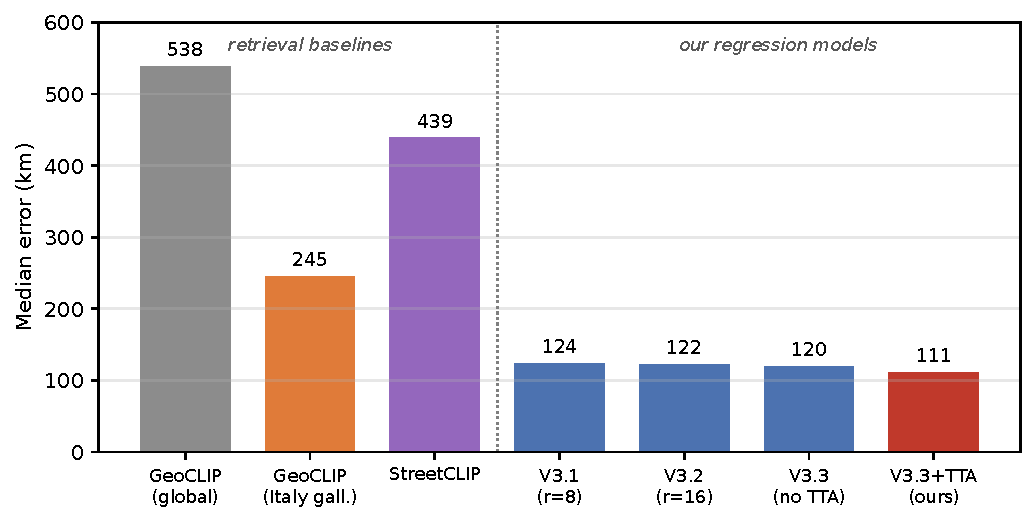
\includegraphics[width=0.99\linewidth]{./charts/ablation_median}
  \caption{Median localization error on the OSV5M test set, all measured by the
  same pipeline. The three retrieval baselines (left) have higher median error
  than all fine-tuned regression models (right); each fine-tuning step adds a
  consistent improvement, with TTA reducing the median error to 111~km.}
  \label{fig:ablation}
\end{figure}

\subsection{Threshold Accuracy and Error Distribution}

Table~\ref{tab:thresholds} gives fine-grained threshold accuracy for the three
baselines and our final model, and Figure~\ref{fig:error_dist} shows the full
error distribution and accuracy-at-distance curves.

\begin{table}[t]
\centering\small
\begin{tabular}{@{}lcccccc@{}}
\toprule
Model & 1 & 25 & 50 & 100 & 200 & 500 \\
\midrule
GeoCLIP (global)   & 0.1 & 3.9  & 6.8  & 14.0 & 24.6 & 47.2 \\
GeoCLIP (Italy)    & 0.1 & 6.8  & 13.3 & 26.8 & 42.8 & 77.5 \\
StreetCLIP         & 0.0 & 0.9  & 2.4  & 5.3  & 16.6 & 60.0 \\
\textbf{V3.3+TTA (ours)} & 0.1 & \textbf{10.6} & \textbf{24.2} & \textbf{45.7} & \textbf{73.6} & \textbf{94.3} \\
\bottomrule
\end{tabular}
\smallskip
\caption{Accuracy (\%) at distance thresholds (km) on the OSV5M test set.}
\label{tab:thresholds}
\end{table}

City-level precision ($\leq$25~km) improves from 3.9\% (global) and 6.8\%
(Italy gallery) to 10.6\%, and province-level ($\leq$100~km) from 14.0\%/26.8\%
to 45.7\%. The 90th-percentile error drops from 1931.9~km (global) to 425.5~km
(ours). The persistent gap at the 1~km street-level threshold suggests that the
512-d globally pooled CLIP representation may not preserve sufficient
fine-grained spatial information for precise localization, discussed further in
\S\ref{sec:limits}.

\begin{figure*}[t]
  \centering
  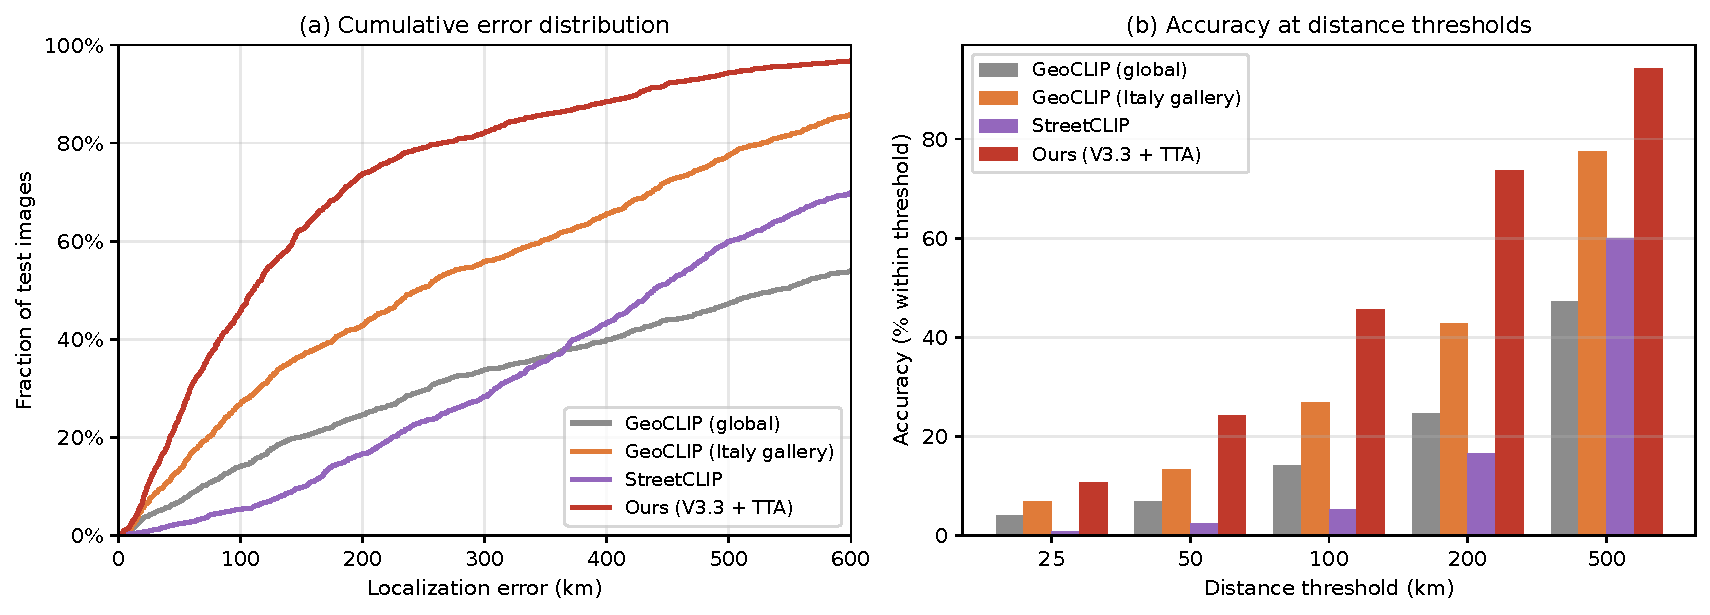
\includegraphics[width=0.99\linewidth]{./charts/cdf_accuracy}
  \caption{(a)~Cumulative error distribution and (b)~accuracy at distance
  thresholds on the OSV5M Italy test set, for the three retrieval baselines and
  our V3.3+TTA model. Our model dominates across the whole error range; the
  largest absolute gains over the Italy-gallery baseline appear in the
  25--200~km band.}
  \label{fig:error_dist}
\end{figure*}

\subsection{Macro-Region Classification}
\label{sec:region}

Assigning each prediction to a macro-region (Nord: lat${>}44.0$; Centro:
$41.5{<}$lat${\leq}44.0$; Sud/Isole otherwise), overall region accuracy rises
from 63.5\% (global baseline) and 66.2\% (Italy gallery) to 80.2\% for V3.3+TTA.
These fixed latitude cutoffs are only a coarse proxy for Italy's administrative
and cultural regions. Sardinia, for instance, spans a wide latitude range, so
assignments near the thresholds may be imprecise.
Table~\ref{tab:region} gives the per-region breakdown against the global
baseline.

\begin{table}[t]
\centering\small
\begin{tabular}{@{}lcccccc@{}}
\toprule
 & \multicolumn{3}{c}{GeoCLIP (global)} & \multicolumn{3}{c}{V3.3 + TTA (ours)} \\
\cmidrule(lr){2-4}\cmidrule(lr){5-7}
Region & P & R & F1 & P & R & F1 \\
\midrule
Nord      & 0.58 & 0.74 & 0.65 & 0.78 & 0.98 & 0.87 \\
Centro    & 0.41 & 0.49 & 0.45 & 0.60 & 0.74 & 0.66 \\
Sud/Isole & 0.82 & 0.65 & 0.73 & 0.96 & 0.75 & 0.84 \\
\midrule
Accuracy  & \multicolumn{3}{c}{0.635} & \multicolumn{3}{c}{\textbf{0.802}} \\
\bottomrule
\end{tabular}
\smallskip
\caption{Macro-region classification on the OSV5M test set (P/R/F1). Test-set
support: Sud/Isole $n{=}734$, Nord $n{=}343$, Centro $n{=}320$.}
\label{tab:region}
\end{table}

Nord achieves very high recall (98.3\%), reflecting the model's stronger
northern training signal, with a per-region median error of 71.7~km.
Sud/Isole has the highest median error, at 159.2~km; this region represents
more than half of the test set but less than a quarter of the training images.
Centro remains the weakest by F1 (0.66): its intermediate latitude overlaps both
neighbors, and the model tends to push ambiguous cases toward the
better-represented Nord.

\subsection{Cross-Dataset Check: IM2GPS3k}
\label{sec:im2gps}

On the landmark-heavy IM2GPS3k Italy subset (\S\ref{sec:im2gps-dataset}) our
model obtains a median error of 106.5~km and a mean error of 152.3~km, but here
the retrieval
baselines perform better at fine spatial scales: GeoCLIP with an Italy gallery
reaches a median error of 21.4~km because many famous monuments are close to
existing gallery cells, and even the global gallery reaches a median error of
32.1~km, although its mean error increases to 762.4~km due to large-error cases.
This suggests a distribution-dependent behavior: retrieval performs better on
iconic landmarks that are close to gallery locations, whereas our model is
optimized for ordinary street-level scenes. The best method depends on the
image distribution, and our target is the everyday-scene regime of OSV5M.

\noindent\textbf{Uncertainty.} Following Gal and Ghahramani~\cite{mcdropout}, MC
Dropout (50 stochastic passes with BatchNorm frozen) yields lower prediction
spread on distinctive urban scenes than on featureless coastal or agricultural
ones, a promising confidence signal, though we have not validated that the
spread correlates with true error, which would be required before deployment.

\subsection{GLDv2 Results for Reference}
\label{sec:gldv2}

For completeness, the two GLDv2-trained versions reached a median error of
168.0~km (V1) and 124.1~km (V2) on the GLDv2 Italy test split, versus 216.0~km
and 235.0~km for their respective GeoCLIP baselines. These numbers are on a
different test set from a landmark-biased dataset and are \emph{not} comparable
to the OSV5M results above; they are reported only to document the progression
that motivated the switch to OSV5M.

\section{Conclusion}

We adapted GeoCLIP to Italy-specific GPS regression by updating only 1.4\% of its
parameters via LoRA on all four ViT-L/14 attention projections, replacing its
gallery-retrieval head with direct coordinate regression.
Evaluated through a single consistent pipeline on the fixed OSV5M test set, our
best model (V3.3+TTA) reduces mean error by 87\% (1290.5$\to$168.0~km) and median
error by 79\% (538.3$\to$110.8~km) versus the pretrained baseline, and still cuts
median error by 55\% against the stronger Italy-gallery baseline, while lifting
macro-region accuracy from 63.5\% to 80.2\%.
A differentiable land-aware penalty is included to discourage open-water
predictions, although its individual contribution is not isolated in the
ablation, and six-view test-time augmentation contributes a final variance
reduction with no retraining.

\noindent\textbf{Limitations and future work.}
\label{sec:limits}
City-level precision remains limited, with only 10.6\% of predictions falling
within 25~km and 0.1\% within 1~km. The model is therefore better suited to
coarse regional localization than to precise GPS estimation. The IM2GPS3k
evaluation indicates that retrieval-based methods remain stronger on iconic
landmark images. Promising extensions include (i)~hierarchical regression
with a coarse region classifier feeding a fine-grained head; (ii)~rebalancing the
Nord-heavy training set via stratified oversampling or loss reweighting;
(iii)~patch-level rather than globally-pooled CLIP features to recover the
spatial detail sub-city precision needs; and (iv)~auxiliary metadata (orientation,
season) as additional regression inputs.

{\small
\bibliographystyle{ieee_fullname}
\bibliography{egbib}
}

\end{document}
